
\documentclass[]{article}

\title{Distribución de probabilidad de normal }

\date{}
\usepackage{braket}
\usepackage{bbold}
\usepackage{amsmath,amsfonts,amssymb,amsthm,booktabs}
\usepackage[margin=1.0in]{geometry}
\usepackage{graphicx}
\usepackage{chngcntr}
\usepackage{floatrow}
\usepackage{chngcntr}
\usepackage{hyperref}
\usepackage[spanish]{babel}
\usepackage[svgnames]{xcolor}
\usepackage{listings}
\usepackage[%
    font={small,sf},
    labelfont=bf,
    format=hang,    
    format=plain,
    margin=0pt,
    width=0.8\textwidth,
]{caption}
\usepackage[list=true]{subcaption}
\lstset{language=R,
    basicstyle=\small\ttfamily,
    stringstyle=\color{DarkGreen},
    otherkeywords={0,1,2,3,4,5,6,7,8,9},
    morekeywords={TRUE,FALSE},
    deletekeywords={data,frame,length,as,character},
    keywordstyle=\color{blue},
    commentstyle=\color{DarkGreen},
}

\counterwithin{figure}{section}
\renewcommand*{\figureautorefname}{Figura}


\usepackage[backend=biber]{biblatex}
\addbibresource{ref.bib}
\begin{document}
	\maketitle
	\begin{center}


\centerline{\textbf{TAREA 5} } 
\textbf{ }

\centerline{Alumno: } 
\centerline{Joaquín Arturo Velarde Moreno}


	\end{center}
	

\section{Introducción}
El objetivo del siguiente reporte es describir el comportamiento de una distribución normal, ver su representación matemática y la forma de su curva en histogramas, para lo cual usaremos el programa R 4.0.2 \cite{rproject} y de este modo, haremos cálculos con conjuntos con la finalidad de mostrarlos gráficamente. Además, intentaremos simular una distribución normal a partir de valores uniformes utilizando la transformación Box-Muller. Para cumplir con esta finalidad, usaremos como apoyo el material de la Dra. Elisa Schaefer \cite{MaterialClase}.


\section{Definición}
La distribución normal o Gaussiana, nombrada así en honor a Carl Friederich Gauss, es una distribución con forma de campana usada para aproximarse al valor de una variable aleatoria continua a una situación ideal. Esta distribución contiene dos parámetros que la definen:$\mu$ y $\sigma$
donde
\begin{itemize}
	\item $\mu$ es la media de la distribución y 
	\item $\sigma$ es la desviación estándar
\end{itemize}
Por ejemplo, si elaboráramos una encuesta de la edad de cada uno de los 150 estudiantes de una escuela y obtuviéramos que su promedio es de 18 años, tendríamos un histograma donde se muestra que hay una mayor cantidad de alumnos cerca del promedio o la media \autoref{fig:Negativo}, es decir, hay la tendencia de querer aproximarse a una curva de distribución normal \autoref{fig:Densidad}.
Pero si esto lo aproximamos a una situación ideal, no tomando la edad de solo 150 individuos sino de 5000 estudiantes, entonces veremos que la forma de nuestra distribución se acerca a la curva de la distribución normal \autoref{fig:Regular}, esta curva nos permite ver dos características de distribución, la asimétrica y la asintótica:


 a)\textbf{Asimétrica} , lo cual significa que la media es igual a los valores de la moda y la mediana, en otras palabras, los alumnos que estén más cerca del promedio, son más numerosos que los que están más alejados de este promedio, esto también implica que se cumple la siguiente ecuación:
 
\[f_X(\mu - x) = f_X(\mu + x) \, \forall x\in \mathbb{R} \]

  
b)	\textbf{Asintótica} , significa que se acerca continuamente a la recta del eje x sin llegar nunca a encontrarla, es decir, puede extenderse hasta el infinito.
La desviación estándar se representa con la letra griega $\sigma$), y nos indica lo lejos que están distribuidos los resultados de la media, lo cual puede producir dos situaciones: una situación homogénea o una heterogénea.

Si la situación es homogénea la desviación estándar $\sigma$ es muy reducida y los sujetos están muy cercanos a la media  $\mu$ y la curva será muy afilada \autoref{fig:Regular}.
En cambio, si la situación es heterogénea la desviación $\sigma$ es muy alta y los sujetos están muy alejados a la media $\mu$ y la curva será menos afilada \autoref{fig:Heterogenea}.


\section{Formula}
La fórmula para la función de probabilidad normal está definida por la siguiente expresión:
\[f_X(x) = \frac{1}{\sigma \sqrt{2\pi }}exp^{(\frac{-(x-\mu)^{2}}{2\sigma^{2} })}\]

donde:
\begin{itemize}
	\item $\mu$ es la media de la distribución.
	\item $\sigma$ es la desviación estándar.
\end{itemize}
Dado que esta ecuación es demasiado complicada, incluso haciendo uso de la calculadora, para este tipo de cálculos se suele hacer uso de la herramienta R \cite{rproject}, en la cual ya está predefinida con la siguiente función \textit{dnorm()}, y si queremos generar un vector de una distribución normal, podemos utilizar el método \textit{rnorm()}.
  \begin{lstlisting}

    Promedio <- 18
    Edad     <- rnorm(500000,Promedio,1)
   \end{lstlisting}

Si esto lo graficamos mediante un histograma, tendremos la misma distribución normal que se espera  \autoref{fig:Regular}
\section{Método de Box-Muller}
También podemos generar una distribución normal por otros métodos tales como el método de Box-Muller, el cual es un método de generación de pares de números aleatorios independientes con distribución normal estándar, es decir con esperanza cero y varianza unitaria, expresada en las siguientes fórmulas.
\[Z_{0} = R\, cos(\Theta ) = \sqrt{-2\, log(U_{1})}\,  cos(2\pi\,  U_{2})\]
\[Z_{1} = R\, sin(\Theta ) = \sqrt{-2\, log(U_{1})}\,  sin(2\pi\,  U_{2})\]

donde:
\begin{itemize}
	\item $U_{1}\, y\, U_{2}$  son variables aleatorias independientes con una distribución uniforme entre los valores 0 a 1.
	\item $Z_{1}\, y\, Z_{2}$ son variables aleatorias independientes con una distribución normal con una desviación estándar
de 1.
\end{itemize}

Esto expresado en R puede ser definido como:
  \begin{lstlisting}
    u = runif(2);
    z0 = sqrt(-2 * log(u[1])) * cos(2 * pi * u[2]);
    z1 = sqrt(-2 * log(u[1])) * sin(2 * pi * u[2]);
   \end{lstlisting}
Si queremos tener nuestra propia media y desviación, podemos afectar la variable aleatoria:
  \begin{lstlisting}
    mu      = 18;
    sigma   = 1;
    u       = runif(2);
    z0      = sqrt(-2 * log(u[1])) * cos(2 * pi * u[2]);
    z1      = sqrt(-2 * log(u[1])) * sin(2 * pi * u[2]);
    z0      = sigma * z0 + mu);
    z1      = sigma * z1 + mu);
   \end{lstlisting}
Si utilizamos este método para generar nuestras variables aleatorias, se obtendrían resultados similares a la distribución normal \autoref{fig:foobar}. 
De esta manera podemos verificar que efectivamente nuestras variables se comportan de acuerdo a una distribución normal teniendo la mayor frecuencia de valores en su media \autoref{fig:boxplot}. 

Es necesario que ambas funciones se obtengan al calcular con dos variables aleatorias de distribución uniforme, en caso de cambiar el cálculo usando únicamente una sola variable uniforme, se rompería la distribución normal  \autoref{fig:singlevariable} .
Esto lo podemos verificar con el método \textit{Shapiro.test()}
el cual nos devuelve un valor \textit{p-value}, si el valor obtenido es mayor a 0.05, entonces significa que nuestro vector muy probablemente viene de una distribución normal, sin embargo este método solo puede trabajar con un vector de 1 a 5000 valores por lo cual, es necesario utilizar el método  \textit{sample()} para tratar con vectores muy grandes.
  \begin{lstlisting}
    test <- shapiro.test(runif(100)) 
    print(test)
    data:  runif(100)
	W = 0.95081, p-value = 0.0009379
	
	# prueba negativa 0.0009379 < 0.05
	                 
    test <- shapiro.test(sample(Edades, 5000, replace = TRUE))
    print(test)
	data:  sample(Edades, 5000, replace = TRUE)
	W = 0.99963, p-value = 0.5049
	
	# prueba positiva 0.5049 > 0.05
   \end{lstlisting}

Si cambiáramos una variable uniforme del método de Box-Muller a por ejemplo esta fuera dependiente de la primera elevándola al cuadrado, también afectaría nuestro distribución \autoref{fig:dependiente} .

  \begin{lstlisting}
   u      <- runif(1);
   u_2    <- u * u;
   z0     <- sqrt(-2 * log(u)) * cos(2 * pi * u_2 );
   z1     <- sqrt(-2 * log(u)) * sin(2 * pi * u_2 );
   datos  <- c(z0, z1);
   \end{lstlisting}

\begin{figure}[b]
    \centering
    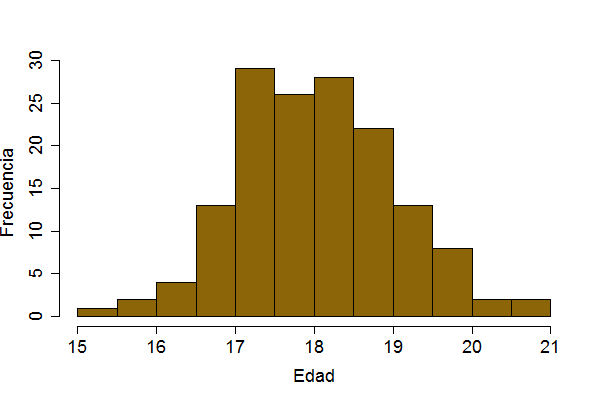
\includegraphics[width=.5\linewidth]{Frecuencia.png}    \caption{Distribución de frecuencia de la encuesta.}
    \label{fig:Negativo}
\end{figure}

\begin{figure}[b]
    \centering
    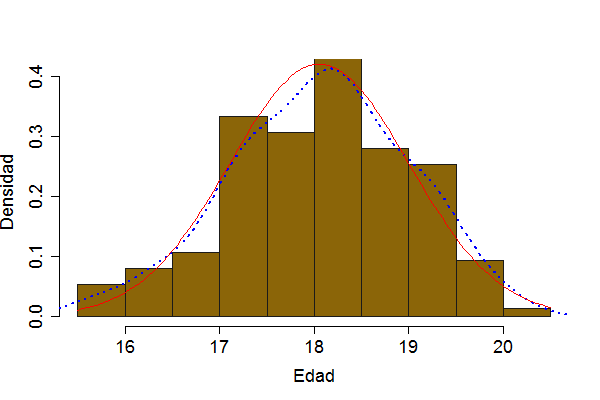
\includegraphics[width=.5\linewidth]{Densidad.png}    \caption{Densidad de resultados en la encuesta.}
    \label{fig:Densidad}
\end{figure}

\begin{figure}[b]
    \centering
    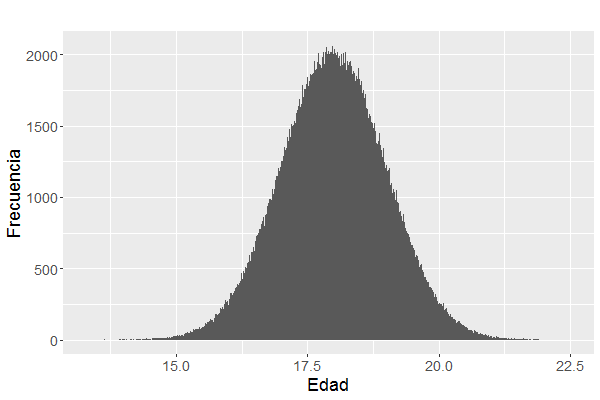
\includegraphics[width=.5\linewidth]{Ideal.png}    \caption{Distribución de frecuencia de la encuesta con 50000 estudiantes.}
    \label{fig:Regular}
\end{figure}

\begin{figure}[b]
    \centering
    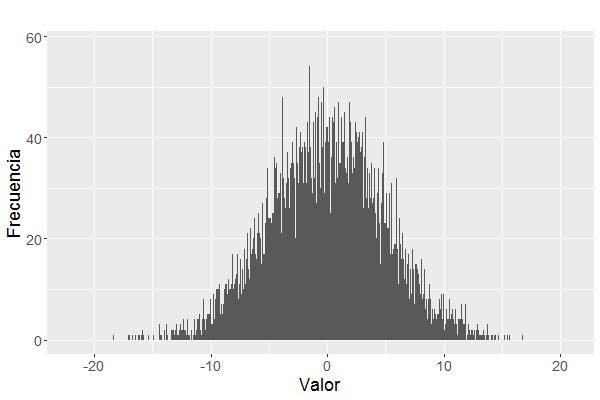
\includegraphics[width=.5\linewidth]{Heterogenea.png}    \caption{Distribución de frecuencia normal heterogénea.}
    \label{fig:Heterogenea}
\end{figure}





\begin{figure}
\centering
\subcaptionbox{Distribución de frecuencia con una sola variable $Z_{1}$.}{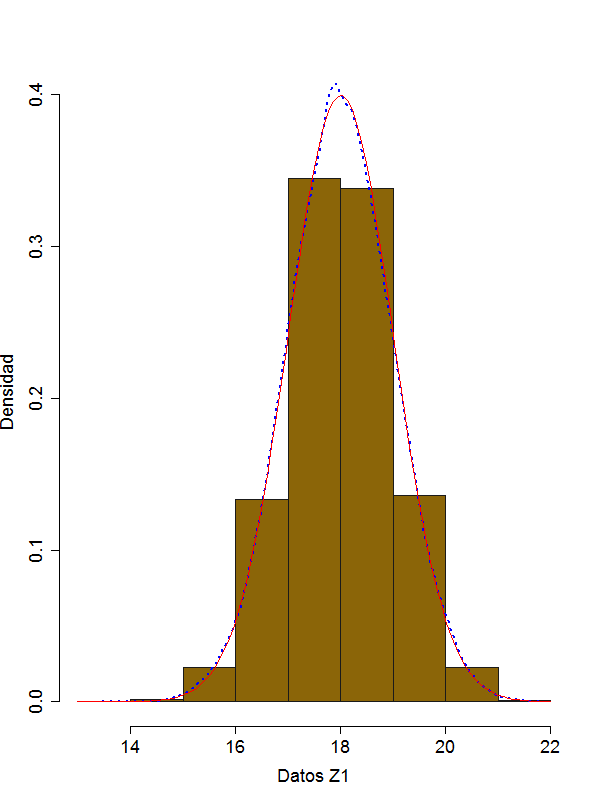
\includegraphics[width=0.3\textwidth]{BoxMuller_z1.png}}%
\hfill
\subcaptionbox{Distribución de frecuencia con una sola variable $Z_{0}$.}{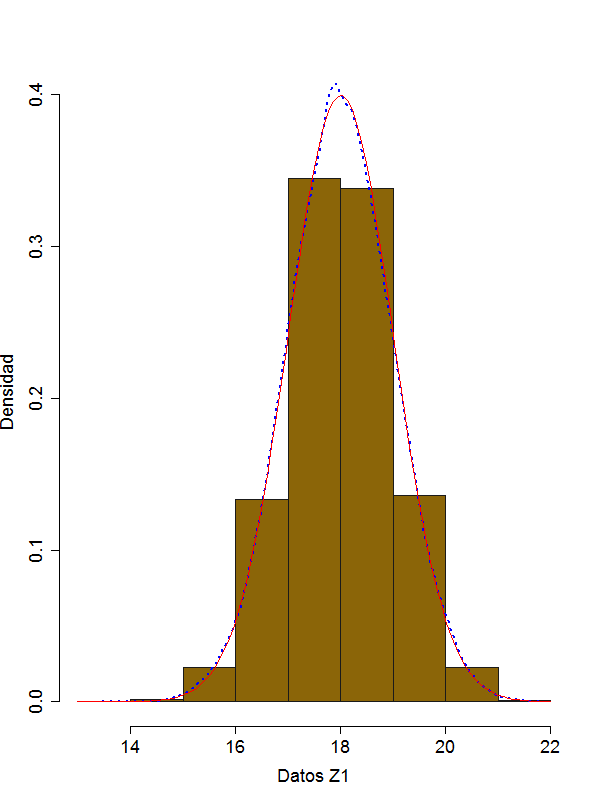
\includegraphics[width=0.3\textwidth]{BoxMuller_z1.png}}%
\hfill
\subcaptionbox{Distribución de frecuencia con ambas variables.}{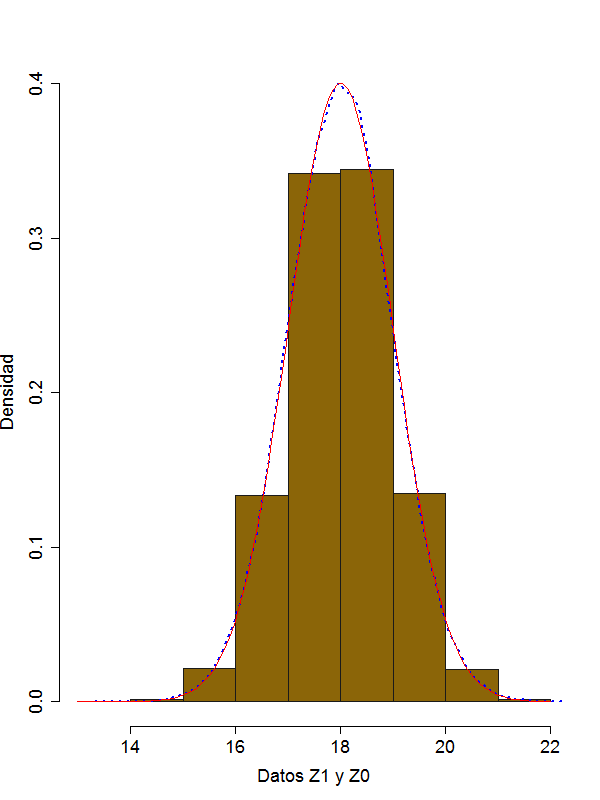
\includegraphics[width=0.3\textwidth]{BoxMuller.png}}%
\hfill
\caption{Densidad de las distribuciones generadas con el método de Box-Muller.}
\label{fig:foobar}
\end{figure}



\begin{figure}[b]
    \centering
    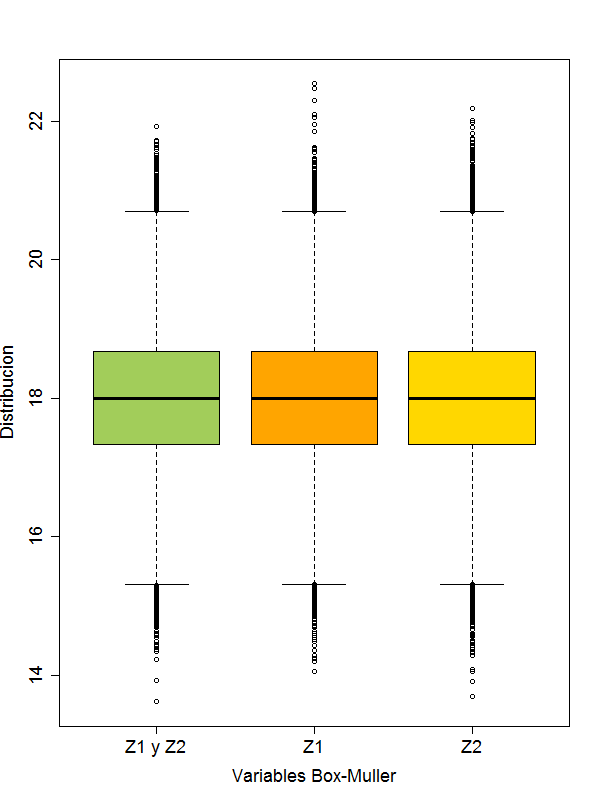
\includegraphics[width=.5\linewidth]{BoxplotVariables.png}    \caption{Distribución de normal de las variables del método Box-Muller por medio de boxplot.}
    \label{fig:boxplot}
\end{figure}









\begin{figure}
\centering
\subcaptionbox{Distribución de frecuencia de la variable $Z_{0} $con solo una variable uniforme.}{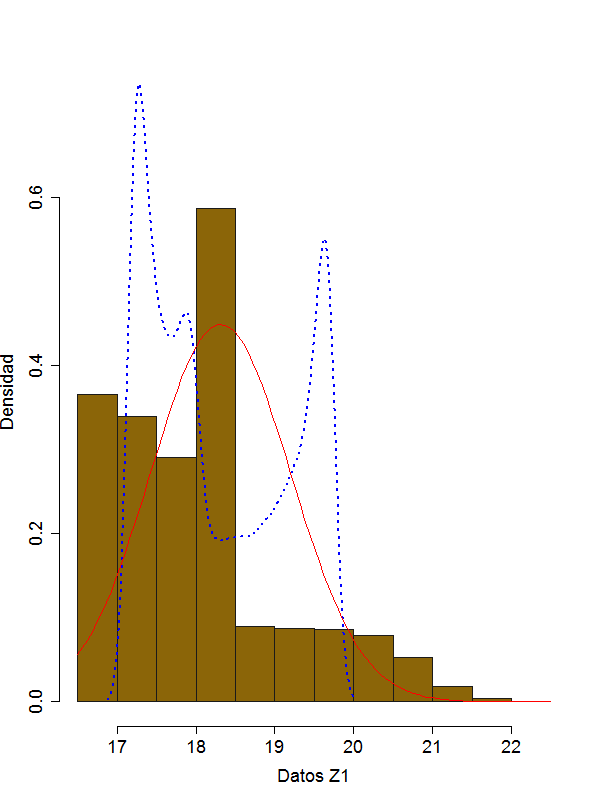
\includegraphics[width=0.4\textwidth]{BoxMuller_z1_variable_2.png}}%
\hfill
\subcaptionbox{Distribución de frecuencia de la variable $Z_{1}$con solo una variable uniforme.}{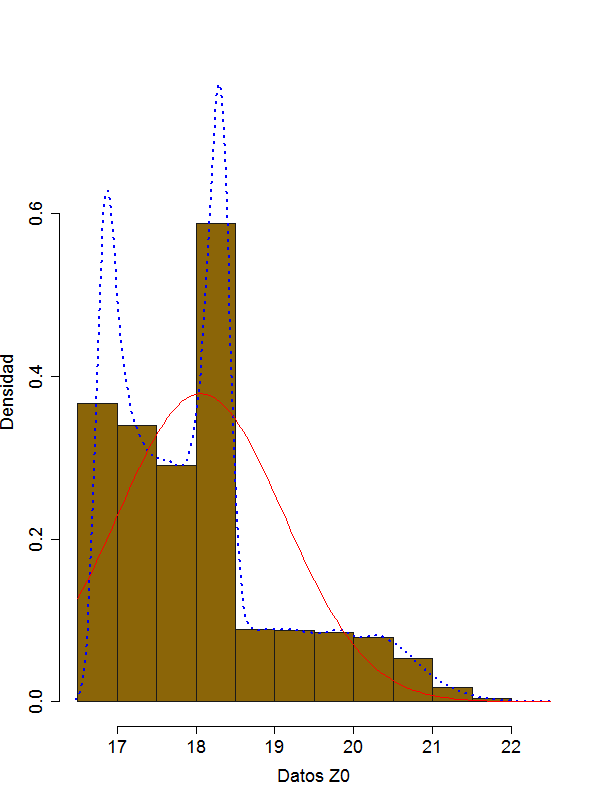
\includegraphics[width=0.4\textwidth]{BoxMuller_z1_variable_1.png}}%
\hfill

\caption{Distribución de frecuencia de la variables de Box-Muller con solo una variable uniforme.}
\label{fig:singlevariable}
\end{figure}





\begin{figure}
\centering
\subcaptionbox{Histograma que muestra la frecuencia de un vector obtenido por el método de Box-Muller.}{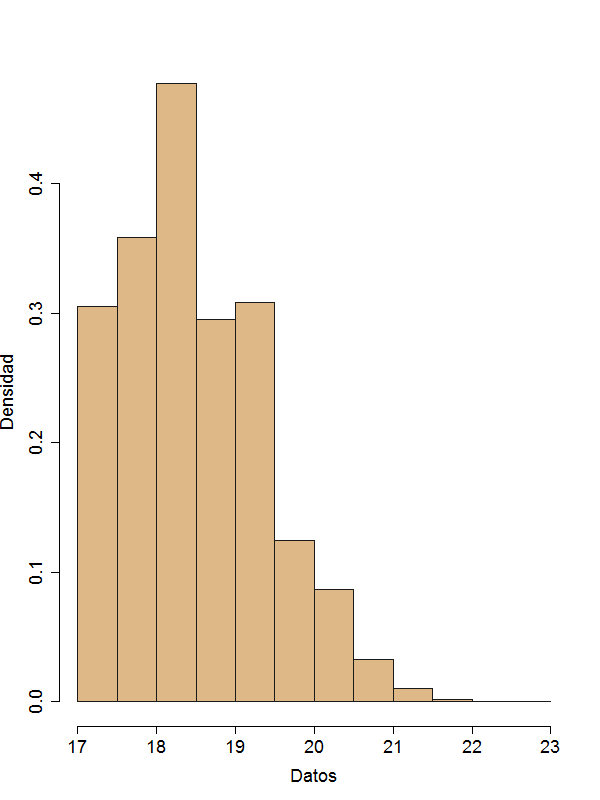
\includegraphics[width=0.4\textwidth]{FrecueciaDependiente.png}}%
\hfill
\subcaptionbox{Densidad de la distribución resultado de una variable dependiente en el método Box-Muller.}{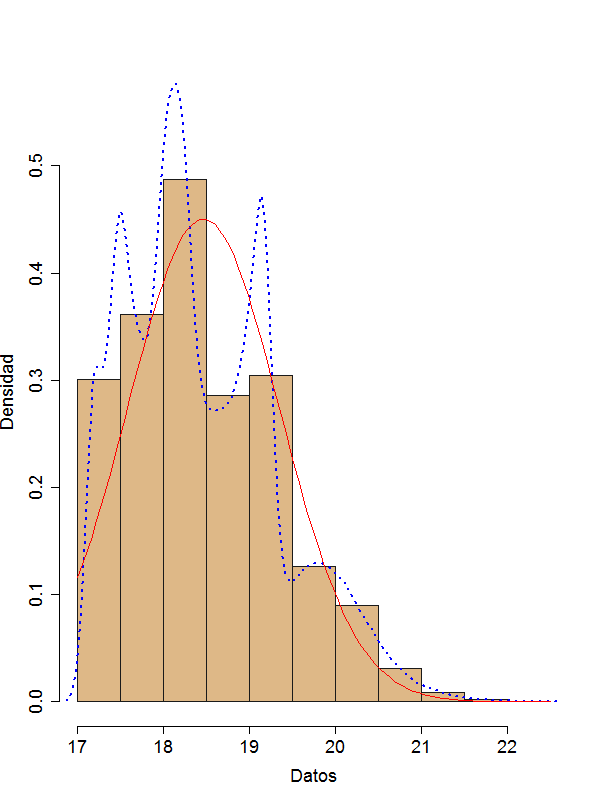
\includegraphics[width=0.4\textwidth]{Dependiente.png}}%
\hfill

\caption{Distribución de frecuencia de los resultados de Box-Muller con una variable uniforme dependiente en una población de 50000 estudiantes.}
\label{fig:dependiente}
\end{figure}








\printbibliography[title={Referencias}]
\end{document}
